\documentclass[UTF8,a4paper]{ctexart}%设置a4纸和中文
\ctexset{section/format=\Large\bfseries}%设置标题左对齐
\usepackage{amsmath} % 使用align
\usepackage[margin=1in]{geometry}%设置A4值的边界
\usepackage{graphicx}%插入图片
\usepackage{amsfonts}%使用bm
\usepackage{color}
\usepackage{amssymb}
\usepackage{bm}
\usepackage{cancel}
\author{qhy}%作者
\title{机器学习笔记4}%标题
\date{\today}%日期
\pagestyle{empty}%不显示页码
\begin{document}
  \maketitle
  \tableofcontents
  \newpage
    \section{隐马尔可夫模型 Hidden Markoy Model HMM}
        {\color{blue}
          之前我们考虑样本之间都是相互独立的,而隐马尔可夫模型则是考虑样本之间不是独立的模型。

          隐马尔可夫模型则是最简单的一种模型。

          概率图模型则是用来描述样本之间的关系的工具。

          隐马尔可夫模型有三个基本问题,分别是评估问题,解码问题,学习问题。前两者可用动态规划算法求解,后者则可以用EM算法求解。

          但是,研究这三个问题的前提是有足够充分的观测空间和状态空间,否则,模型的泛华能力将会很弱。
          但是足够充分的空间,也意味着更大的时间开销。从时间来看,隐马尔可夫模型的时间开销会很巨大。
        }
        \subsection{概率图模型}
            \textbf{概率图模型 probabilistic graphical model}是一类用图来表达变量相关关系的概率模型。
            它以图为表示工具,最常见的是用一个结点表示一个或一组随机变量,结点之间的边表示变量间的概率相关关系,即"变量关系图"。

            根据边的性质不同,概率图模型可大致分为两类:
            \begin{itemize}
              \item 有向图模型(贝叶斯网 Bayesian network)

                  使用有向无环图表示变量间的依赖关系

                  {\color{blue}
                      隐马尔可夫模型(HMM) 是结构最简单的动态贝叶斯网。
                  }

              \item 无向图模型(马尔可夫网 Markov network)

                  使用无向图表示变量间的相关关系。

            \end{itemize}
        \subsection{隐马尔可夫模型}
            \textbf{隐马尔可夫模型}:隐马尔可夫模型是关于时序的概率模型,描述由一个隐藏的马尔可夫链随机生成不可观测的状态随机序列,再由各个状态生成一个观测而产生观测随机序列的过程。

            马尔可夫链:系统下一时刻的状态仅由当前状态决定,不依赖以往的任何状态。

            隐马尔可夫模型是一个生成模型。

            隐马尔可夫模型中的变量可分为两组:
            \begin{itemize}
              \item 状态变量 (隐变量)

                  状态变量:$\{y_1, y_2 , \cdots , y_n\}$,其中$y_i \in \mathcal{Y} $表示第i个时刻的系统状态。\\
                  通常假定状态变量是隐藏的、不可被观测的,因此状态变量亦称\textbf{隐变量(hidden variable)}

              \item 观测变量

                  观测变量:$\{x_1, x_2 , \cdots , x_n\}$,其中$x_i \in \mathcal{X} $表示第i个时刻的观测值。
            \end{itemize}

            状态空间:$\mathcal{Y} = \{s_1,s_2,\cdots , s_N\}$,其中$s_i$表示一个具体的状态

            观测空间:$\mathcal{X} = \{o_1,o_2,\cdots , o_M\}$,其中$o_i$表示一个具体的观测值

            参数定义:$\lambda = \{\bm{A,B,\pi}\}$
            \begin{itemize}
              \item 状态转移概率

                  模型在各个状态之间转换的概率 , 通常记为矩阵 $\bm{A} = [a_{ij}]_{N\times N}$,其中
                  \[ a_{ij} = P(y_{t+1} = s_j | y_t = s_i) , 1 \leqslant i,j \leqslant N , {\color{red} \forall t }\]

                  表示在任意t时刻,若状态为$s_i$,则在下一个时刻状态为$s_j$的概率

              \item 输出观测概率

                  模型根据当前状态获得各个观测值的概率,通常记为矩阵$\bm{B} = [b_{ik}]_{N\times M}$,其中
                  \[ b_{ik} = P(x_t = o_k | y_t = s_i)  ,1 \leqslant i \leqslant N ,1 \leqslant k \leqslant M ,{\color{red} \forall t }\]

                  表示在任意时刻t,若状态为$s_i$,则观测值$o_j$被获取的概率

              \item 初始状态概率

                  模型在初始时刻各状态出现的概率,通常记为$\bm{\pi} = (\pi_1 , \pi_2 , \cdots ,\pi_N)$,其中
                  \[ \pi_i = P(y_1 = s_i) , 1 \leqslant i \leqslant N \]

                  表示模型初始状态为$s_i$的概率
            \end{itemize}

            图\ref{statusstransferfig}是状态转移图
            \begin{figure}[!htbp]
              \centering
              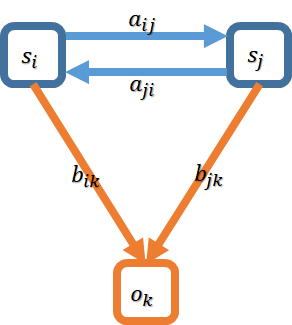
\includegraphics[scale=0.5]{assets/jiqixuexi4_85f62.png}
              \caption{状态转移图,$a_{ij}$表示从状态$s_i$转移到状态$s_j$的概率,$b{i_k}$表示状态$s_i$下观测值$o_k$被获取的概率}
              \label{statusstransferfig}
            \end{figure}

            给定状态空间$\mathcal{Y}$ , 观测空间$\mathcal{X}$ , 参数$\lambda$ , 就能确定一个隐马尔可夫模型。

            \textbf{下面是给定$\lambda$下,模型产生观测序列$\{x_1, x_2, \cdots , x_n\}$的过程(见图\ref{generationOfHMM}):}

            {\color{blue}
              由初始状态触发,由状态转移方程不断驱动。
            }

            \begin{tabular}{l}
              \hline
              (1): 设置$t=1$,并根据初始状态概率$\bm{\pi}$选择初始状态$y_1$\\
              (2): 根据状态$y_t$和观测概率$\bm{B}$选择观测变量值$x_t$\\
              (3): 根据状态$y_t$和状态转移矩阵$\bm{A}$转移模型状态,即确定$y_{t+1}$\\
              (4): 若$t<n$,设置$t=t+1$,并转到第(2)步,否则停止\\
              \hline
            \end{tabular}

            \begin{figure}[!htbp]
              \centering
              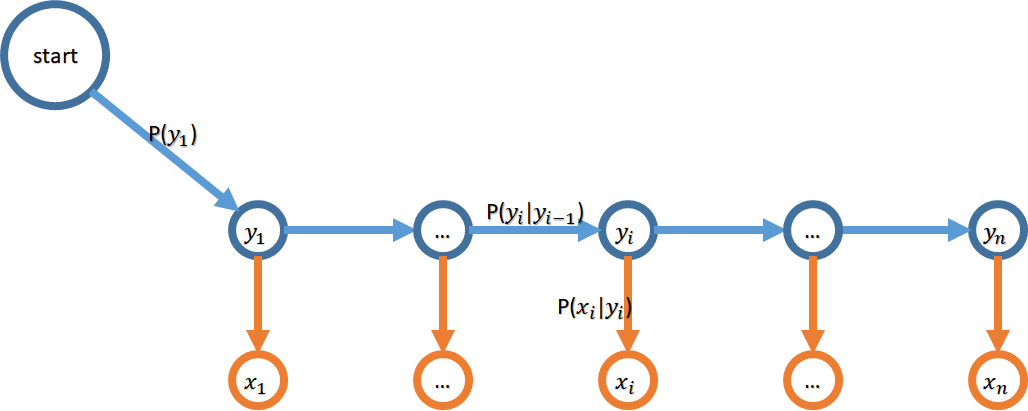
\includegraphics[scale=0.4]{assets/jiqixuexi4_06c36.png}
              \caption{隐马尔可夫模型的图结构}
              \label{generationOfHMM}
            \end{figure}

            在实际应用中,人们常关注隐马尔可夫模型的三个基本问题:
            \begin{itemize}
              \item 评估问题/预测问题

                  给定模型参数$\lambda = \{\bm{A,B,\pi}\}$,如何有效计算其产生观测序列$\{x_1, x_2, \cdots , x_n\}$ 的概率$P(\bm{x} | \lambda)$?换言之,如何评估模型与观测序列之间的匹配程度?

                  {\color{blue}

                  评估问题,具体来说,就是计算观测样本的出现的概率,这个概率的主要用于三个方面:

                  \begin{itemize}
                    \item [1.] 用于预测下一个最可能出现的观测值

                          给定$\{x_1, x_2, \cdots , x_{n-1}\}$预测$x_n$,即在不同$x_n$下,求$P(\bm{x} | \lambda)$,取概率最大的$x_n$,即
                              \[ x_n^* = arg \max_{x_n} P(\bm{x} | \lambda) \]

                    \item [2.] 用来评价当前序列对应的模型和我们猜测的模型的匹配程度

                          如果匹配的话,则观测序列出现的概率应该会比较大(极大似然法的思想)

                          如果使用我们猜测的模型参数计算出来的观测序列的概率大,我们就有理由相信这个序列有可能是由这个模型产生的。{\color{red},但是,这个判断的阈值具体取多少,不知道这里是否一个评价的标准。}

                          具体的例子:骰子产生的序列和骰子有关系,但是如果骰子被庄家都手脚了,那么,出现的序列有更大的可能性对庄家有利,也就是说如果出现大部分的序列都是对买家有利的,我们就有理由相信骰子被动过手脚。(这里假设有多个骰子,隐变量是选择了哪个骰子,每个骰子选中的概率一样,虽然这个隐变量实际上并没有什么作用,但却和隐马尔可夫模型建立了关系,可以用隐马尔可夫模型求解,也可以看成是状态空间只有一个状态的隐马尔科夫模型)\\

                    \item [3.] 用于EM算法过程的计算
                  \end{itemize}
                  }

              \item 解码问题

                  给定模型参数$\lambda = \{\bm{A,B,\pi}\}$和观测序列$\{x_1, x_2, \cdots , x_n\}$,如何找到与此观测序列最匹配的状态序列$\{y_1,y_2 , \cdots , y_n\}$?换言之,如何根据观测序列推断出隐藏的模型状态?

                  {\color{blue}
                      在语音识别中,观测值为语音信号,隐藏状态为文字,目标就是根据观测信号来推断最有可能的状态序列(即对应的文字)
                  }

              \item 学习问题

                  给定观测序列$\{x_1, x_2, \cdots , x_n\}$

                  如何调整模型参数$\lambda = \{\bm{A,B,\pi}\}$ 使得该序列出现的概率$P(\bm{x} | \lambda)$最大?换言之,如何训练模型使其能很好地描述观测数据?

            \end{itemize}


            {\color{blue}
                三个问题分别对应于观测变量$\{x_1,x_2,\cdot x_n\}$,状态变量$\{y_1,y_2 , \cdots , y_n\}$和参数$\lambda = \{\bm{A,B,\pi}\}$
            }

        \subsection{基本问题1-评估问题}
            给定模型参数$\lambda = \{\bm{A,B,\pi}\}$,如何有效计算其产生观测序列$\{x_1, x_2, \cdots , x_n\}$(简记为$\bm{x} = x_{1:n}$) 的概率$P(\bm{x} | \lambda)$?换言之,如何评估模型与观测序列之间的匹配程度?

            首先,在已知$\bm{y} = y_{1:n} = \{y_1, y_2 , \cdots , y_n \}$时的概率:

            {\color{blue}
              状态$x_{1:n}$由$x_{1:n-1}$经过$y_{n-1}\to y_{n} \to x_{n}$两步得到。
            }
            \begin{equation}\begin{split}
              P(\bm{x,y}|\lambda) &= P(x_{1:n},y_{1:n} | \lambda)\\
              &= P(x_{1:n-1},y_{1:n-1} | \lambda)P(y_{n}|y_{n-1})P(x_n|y_{n})\\
              &= P(y_1)P(x_1|y_1)\prod_{i = 2}^n P(y_{i}|y_{i-1})P(x_i|y_{i})
            \end{split}\end{equation}

            为方便,记$P(y_1|y_0) = P(y_1)$($y_0$不存在),则上面公式可以写成:
            \begin{equation}
              P(\bm{x,y}|\lambda) = \prod_{i = 1}^n P(y_{i}|y_{i-1})P(x_i|y_{i})
            \end{equation}

            则由全概率公式
            \begin{equation}\begin{split}
                P(\bm{x}|\lambda) &= \sum_{\bm{y}}P(\bm{x,y}|\lambda) \\
                &= \sum_{\bm{y}} \prod_{i = 1}^n P(y_{i}|y_{i-1})P(x_i|y_{i})
            \end{split}\end{equation}

            求$P(\bm{x,y}|\lambda)$耗时$O(n)$,而$\bm{y}$有$N^n$种组合,

            则计算 $P(\bm{x}|\lambda)$的时间代价为{\color{red}$O(nN^n)$},指数复杂度,显然是不可接受的

            下面介绍计算$P(\bm{x}|\lambda)$的有效算法:前向-后向算法

            {\color{blue}
                前向算法的本质是动态规划算法。

                而前向算法和后向算法则是同一种动态规划算法在不同方向上的实现。
            }


            图\ref{fig2017-5-1819:40:09}是概率计算示意图。

            每一条路径表示一个可能的选择,由全概率公式,总的概率就是所有路径对应的概率之和 。

            从第一列和第二列来看,两列的任意组合是三列组合的一个公共因子。

            前面直接展开运算的结果,就是对这个公共因子进行的多次重复的计算。

            前向-后向算法则是把这些重复运算的结果保存起来的一个动态规划算法。

            \begin{figure}[!htbp]
              \centering
              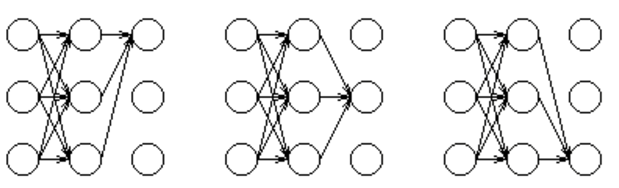
\includegraphics[scale=0.5]{assets/jiqixuexi4_36b94.png}
              \caption{前向后向算法概率计算示意图}
              \label{fig2017-5-1819:40:09}
            \end{figure}

            \begin{itemize}
              \item 前向算法

                  \textbf{定义(前向概率)}:给定隐马尔可夫模型的参数$\lambda$
                  到$t$时刻的观测序列为$\{x_1,x_2 , \cdots , x_t\}$(简记为$x_{1:t}$),时刻$t$的状态为$s_i$,定义$t$时刻的前向概率为:

                  \begin{equation}
                    \alpha_t(i) = P(x_{1:t},y_t = s_i|\lambda)
                  \end{equation}

                  则$t+1$时刻的前向概率为:
                  \begin{equation}
                    \alpha_{t+1}(i) = \left ( \sum_{j =1}^N \alpha_t(j)P(y_{t+1} = s_i|y_t = s_j,\lambda) \right ) P(x_{t+1}|y_{t+1} = s_i,\lambda)
                  \end{equation}

                  初始条件:
                  $\alpha_1(i) = \pi_iP(x_1 |y_1 = s_i)$

                  则序列$\{x_1,x_2 , \cdots , x_n\}$的概率就是时刻$n$的所有前向概率之和:
                  \begin{equation}
                    P(\bm{x}|\lambda) = \sum_{i = 1}^N \alpha_n(i)
                  \end{equation}

              \item 后向算法

                  \textbf{定义(后向概率)}:给定隐马尔可夫模型的参数$\lambda$,时刻$t$的状态为$s_i$,从$t+1$时刻到最后时刻$n$的部分观测序列为$\{x_{t+1},x_{t+2} , \cdots , x_n\}$(简记为$x_{t+1:n}$),则时刻t的后向概率为:
                  \begin{equation}
                    \beta_t(i) = P(x_{t+1:n}|y_t = s_i , \lambda)
                  \end{equation}

                  则$t-1$时刻的后向概率为:
                  \begin{equation}
                    \beta_{t-1}(i) = \sum_{j = 1}^N \beta_{t}(j)P(y_{t} = s_j|y_{t-1} = s_i,\lambda)P(x_{t-1}|y_{t-1} = s_i,\lambda)
                  \end{equation}

                  初始条件:
                  $\beta_n(i) = 1,\forall 1 \leqslant i \leqslant N$

                  则序列$\{x_1,x_2 , \cdots , x_n\}$的概率就是时刻$0$的所有后向概率之和:

                  {\color{blue}
                      时刻0是不存在的,从时刻1开始计算,这里为描述方便,说成时刻0,也就是
                      $\{x_{1},x_{2} , \cdots , x_n\}$的后向概率。
                  }

                  \begin{equation}
                    P(\bm{x}|\lambda) = \sum_{i = 1}^N \pi_iP(x_1|y_1 = s_i,\lambda)\beta_1(i)
                  \end{equation}

              \item 前向后向算法(二合一)
                  \begin{equation}\begin{split}
                    P(\bm{x}|\lambda) &= \sum_{i = 1}^N \alpha_t(i) \beta_t(i)\\
                    &= \sum_{i = 1}^N \sum_{j = 1}^N \alpha_t(i) a_{i,j} b_j(x_{t+1}) \beta_{t+1}(j) \\&\quad \forall t \in [1,n)]
                  \end{split}\end{equation}

                  {\color{blue}
                    第一个等式枚举任意一个时刻的状态

                    第二个等式枚举任意两个相邻时刻的状态
                  }
            \end{itemize}

        \subsection{基本问题2-解码问题}
            给定模型参数$\lambda = \{\bm{A,B,\pi}\}$和观测序列$\{x_1, x_2, \cdots , x_n\}$(简记为$x_{1:n}$),如何找到与此观测序列最匹配的状态序列$\{y_1,y_2 , \cdots , y_n\}$(简记为$y_{1:n}$)?换言之,如何根据观测序列推断出隐藏的模型状态?

            解决这个问题,需要使用\textbf{Viterbi 算法}

            {\color{blue}
            \textbf{Viterbi 算法}也是一个动态规划算法:首先求最优值(该观测序列概率的最大值,针对不同的状态序列,观测序列的概率不一样),然后根据最优值还原最优解
            }

            \textbf{Viterbi 算法}:

            对于观测序列$x_{1:n}$,定义$V_{t,k}$表示到时刻t为止,且时刻t的状态为$s_k$的最大概率,

            即$V_{t,k} = \max_{y_{1:t-1}} P(\bm{x_{1:t}}|\lambda,y_{1:t-1} , y_t = s_k)$

            {\color{blue}
                区别于\textbf{基本问题1} , 前者是隐变量随机的时候的概率,后者是针对某一个特定的状态序列的概率
            }

            则有以下递推关系:
            \begin{equation}
                V_{t,k} = \begin{cases}
                  P(x_1|y_1 = s_k)\pi_k &,t = 1\\
                  P(x_t|y_t = s_k)\max_{s_i \in \mathcal{Y}}\left(P(y_t = s_k|y_{t-1} = s_i)V_{t-1,s_i}\right) &,t > 1
              \end{cases}
            \end{equation}

            还原最优解:
            $y_{t} = \begin{cases}
            arg \max_{s_i \in \mathcal{Y}}\left(P(y_{t+1}|y_{t} = s_i)V_{t,s_i}\right) & , t < n\\
            arg \max_{s_i \in \mathcal{Y}} V_{t,s_i} &, t = n
            \end{cases}, t:n \to 1$

            {\color{blue}
                每一步递推,都是选择概率乘积的最大值,即$\max_{s_i \in \mathcal{Y}}\left(P(y_t = s_k|y_{t-1} = s_i)V_{t-1,s_i}\right)$,这一步选择的状态(上一个时刻的状态),就是最大化概率的状态
            }

        \subsection{基本问题3-学习问题}

            给定观测序列$\bm{x} = \{x_1, x_2, \cdots , x_n\}$

            如何调整模型参数$\lambda = \{\bm{A,B,\pi}\}$ 使得该序列出现的概率$P(\bm{x} | \lambda)$最大?换言之,如何训练模型使其能很好地描述观测数据?

            {\color{blue}
                含隐变量的参数估计,可以用EM算法。
            }

            给定观测序列$\bm{x}$和状态序列$\bm{y}$,则对数似然函数为:
            \begin{equation}
              \begin{split}
              LL(\lambda|\bm{x,y}) &= \ln P(\bm{x,y}|\lambda) \\
                &= \ln P(y_1)P(x_1|y_1)\prod_{i = 2}^n P(y_i|y_{i - 1})P(x_i | y_i) \\
                &= \ln P(y_1) + \sum_{i = 2}^n \ln P(y_i|y_{i-1}) + \sum_{i = 1}^n \ln P(x_i|y_i)\\
                &= \ln P(y_1) + \sum_{i = 1}^{n-1} \ln P(y_{i+1}|y_{i}) + \sum_{i = 1}^n \ln P(x_i|y_i)
            \end{split}
            \end{equation}

            根据EM算法,每次迭代优化目标为:
            $\lambda = arg \max_{\lambda} Q(\lambda , \hat{\lambda}) = arg \max_{\lambda} \sum_{\bm{y}} P(\bm{y}|\bm{x},\hat{\lambda})P(\bm{x,y}|\lambda)$

            {\color{red}
            在统计学习方法一书中,在进行EM算法的推导的时候,乘上了一个常数因子$P(\bm{x}|\hat{\lambda})$,不知道有什么深意。
            }

            \sout{优化目标乘上一个常数$P(\bm{x}|\hat{\lambda})$,则优化目标等价于}
              \[ \cancel{\lambda = arg \max_{\lambda} \sum_{\bm{y}} P(\bm{x}|\hat{\lambda})P(\bm{y}|\bm{x},\hat{\lambda})P(\bm{x,y}|\lambda) = arg \max_{\lambda} \sum_{\bm{y}} P(\bm{x,y}|\hat{\lambda})P(\bm{x,y}|\lambda)} \]

            \sout{记:}$\cancel{Q'(\lambda,\hat{\lambda}) = \sum_{\bm{y}} P(\bm{x,y}|\hat{\lambda})P(\bm{x,y}|\lambda)}$

            \begin{align}
              Q(\lambda,\hat{\lambda}) &= \sum_{\bm{y}} P(\bm{y}|\bm{x},\hat{\lambda})P(\bm{x,y}|\lambda)\\
                &= \sum_{y} P(\bm{y}|\bm{x},\hat{\lambda}) \left( \ln P(y_1) + \sum_{i = 1}^{n-1} \ln P(y_{i+1}|y_{i}) + \sum_{i = 1}^n \ln P(x_i|y_i) \right )\\
                &= \sum_{\bm{y}} P(\bm{y}|\bm{x},\hat{\lambda}) \ln P(y_1)
                  + \sum_{\bm{y}} P(\bm{y}|\bm{x},\hat{\lambda})  \sum_{i = 1}^{n-1} \ln P(y_{i+1}|y_{i})\\
                  &\quad + \sum_{\bm{y}} P(\bm{y}|\bm{x},\hat{\lambda}) \sum_{i = 1}^n \ln P(x_i|y_i) \notag \\
                &= {\color{red}
                \sum_{i = 1}^N  P(y_1 = s_i|\bm{x},\hat{\lambda}) \ln P(y_1 = s_i)}\label{eq-2017-5-1819:56:52}\\
                  &\quad{\color{red}
                  + \sum_{i = 1}^N \sum_{j = 1}^N \sum_{t = 1}^{n-1}
                       P(y_t = s_i , y_{t+1} = s_j|\bm{x},\hat{\lambda}) \ln P(y_{t+1} = s_j|y_{t} = s_i)} \notag \\
                  &\quad{\color{red}
                   + \sum_{i = 1}^N \sum_{t = 1}^n P(y_t = s_i|\bm{x},\hat{\lambda}) \ln P(x_t|y_t = s_i)} \notag \\
                &= \sum_{i = 1}^N  P(y_1 = s_i|\bm{x},\hat{\lambda}) \ln \pi_i\\
                  &\quad+ \sum_{i = 1}^N \sum_{j = 1}^N \sum_{t = 1}^{n-1}
                      P(y_t = s_i , y_{t+1} = s_j|\bm{x},\hat{\lambda}) \ln a_{ij} \notag\\
                  &\quad + \sum_{i = 1}^N \sum_{t = 1}^n P(y_t = s_i|\bm{x},\hat{\lambda}) \ln b_i(x_t) \notag
            \end{align}

            {\color{blue}
            式\eqref{eq-2017-5-1819:56:52}是对公式的一个具体展开。

            \begin{equation}
              \begin{split}
              \sum_{\bm{y}} P(\bm{y}|\bm{x},\hat{\lambda}) \ln P(y_1) &= \sum_{y_1} \sum_{y_{2:n}}
              P(y_1, y_{2:n}|\bm{x},\hat{\lambda}) \ln P(y_1) \\
              &= \sum_{y_1} \sum_{y_{2:n}}
              P(y_1|\bm{x},\hat{\lambda})P(y_{2:n}|y_1,\bm{x},\hat{\lambda}) \ln P(y_1)\\
              &= \sum_{y_1}
              \left ( \sum_{y_{2:n}} P(y_{2:n}|y_1,\bm{x},\hat{\lambda}) \right ) P(y_1|\bm{x},\hat{\lambda}) \ln P(y_1) \\
              &= \sum_{i = 1}^N  P(y_1 = s_i|\bm{x},\hat{\lambda}) \ln P(y_1 = s_i)
            \end{split}
            \end{equation}
            }


            \textbf{求$\bm{\pi}$}

            由拉格朗日乘数法($\sum_{i= 1}^N \pi_i = 1$):
            \begin{equation}
              \frac{\partial\left( Q'(\lambda,\hat{\lambda}) + \lambda\left( \sum_{j = 1}^N \pi_j - 1\right) \right)}{\partial \pi_i} = 0
            \end{equation}
            得到:
            \begin{equation}
              P(y_1 = s_i|\bm{x},\hat{\lambda}) + \lambda \pi_i = 0
              \label{eq-2017-5-1722:28:47}
            \end{equation}
            对所有$N$个$\pi_i$累加,得到:
            \begin{equation}
              \begin{split}
              \sum_{i = 1}^N P(y_1 = s_i|\bm{x},\hat{\lambda}) + \lambda = 0\\
              1 + \lambda = 0
              \end{split}
            \end{equation}
            代入式\eqref{eq-2017-5-1722:28:47}得:
            \begin{equation}
              \pi_i = P(y_1 = s_i|\bm{x},\hat{\lambda})
            \end{equation}

            \textbf{求$\bm{A}$}

            由拉格朗日乘数法($\sum_{j = 1}^N a_{i,j} = 1$):
            \begin{equation}
              \frac{\partial\left( Q'(\lambda,\hat{\lambda}) + \lambda\left( \sum_{k = 1}^N a_{i,k} - 1 \right) \right)}{\partial a_{i,j}} = 0
            \end{equation}
            得到:
            \begin{equation}
              \sum_{t = 1}^{n-1}
                  P(y_t = s_i , y_{t+1} = s_j|\bm{x},\hat{\lambda})  + \lambda a_{i,j} = 0
              \label{eq-2017-5-1722:35:38}
            \end{equation}
            对所有$N$个$a_{i,j}$累加,得到:
            \begin{equation}
              \sum_{k = 1}^N \sum_{t = 1}^{n-1}
                  P(y_t = s_i , y_{t+1} = s_k|\bm{x},\hat{\lambda})  + \lambda = 0
            \end{equation}
            代入式\eqref{eq-2017-5-1722:35:38}得:
            \begin{equation}
              \begin{split}
              a_{i,j} &= \frac{ \sum_{t = 1}^{n-1}
                  P(y_t = s_i , y_{t+1} = s_j|\bm{x},\hat{\lambda}) }{\sum_{k = 1}^N \sum_{t = 1}^{n-1}
                  P(y_t = s_i , y_{t+1} = s_k|\bm{x},\hat{\lambda})}\\
                  &= \frac{ \sum_{t = 1}^{n-1}
                      P(y_t = s_i , y_{t+1} = s_j|\bm{x},\hat{\lambda}) }{ \sum_{t = 1}^{n-1}
                      P(y_t = s_i|\bm{x},\hat{\lambda})}
                \end{split}
            \end{equation}

            \textbf{求$\bm{B}$}

            由拉格朗日乘数法($\sum_{k = 1}^N b_{i,k} = 1;b_{i,k} = b_i(x = o_k)$):
            \begin{equation}
              \frac{\partial\left( Q'(\lambda,\hat{\lambda}) + \lambda\left( \sum_{j = 1}^N b_{i,j}  - 1 \right) \right)}{\partial b_{i,k}} = 0
            \end{equation}
            得到:
            \begin{equation}
               \sum_{t = 1}^n P(y_t = s_i|\bm{x},\hat{\lambda})I(x_t = o_k)  + \lambda b_{i,k} = 0
              \label{2017-5-1722:44:14}
            \end{equation}
            对所有$N$个$b_{i,k}$累加,得到:
            \begin{equation}
              \sum_{j = 1}^N \sum_{t = 1}^n P(y_t = s_i|\bm{x},\hat{\lambda})I(x_t = o_j)  + \lambda = 0
            \end{equation}
            代入式\eqref{2017-5-1722:44:14}得:
            \begin{equation}
              \begin{split}
              b_{i,k} &= \frac{\sum_{t = 1}^n P(y_t = s_i|\bm{x},\hat{\lambda})I(x_t = o_k)}
                  {\sum_{j = 1}^N \sum_{t = 1}^n P(y_t = s_i|\bm{x},\hat{\lambda})I(x_t = o_j)}\\
              &= \frac{\sum_{t = 1}^n P(y_t = s_i|\bm{x},\hat{\lambda})I(x_t = o_k)}
              { \sum_{t = 1}^n P(y_t = s_i|\bm{x},\hat{\lambda})}
            \end{split}
            \end{equation}

            可以用前向-后向算法来计算$P(y_t = s_i|\bm{x},\hat{\lambda})$和$P(y_t = s_i , y_{t+1} = s_j|\bm{x},\hat{\lambda})$

            \begin{equation}
              \begin{split}
              P(y_t = s_i|\bm{x},\hat{\lambda}) &= \frac{P(\bm{x},y_t = s_i|\hat{\lambda})}
                {P(\bm{x}|\hat{\lambda})} \\
                &= \frac{\alpha_t(i)\beta_t(i)}{\sum_{i = 1}^N \alpha_t(i) \beta_t(i)}
              \end{split}
            \end{equation}

            \begin{equation}
              \begin{split}
              P(y_t = s_i , y_{t+1} = s_j|\bm{x},\hat{\lambda})
              &= \frac{  P(y_t = s_i , y_{t+1} = s_j,\bm{x}|\hat{\lambda})}{  P(\bm{x}|\hat{\lambda})}\\
              &= \frac{\alpha_t(i)a_{i,j}b_j(x_{t+1})\beta_{t+1}(j)}{\sum_{i = 1}^N \alpha_t(i) \beta_t(i)}
            \end{split}
            \end{equation}

            为方便,记
            \[\gamma_t(i) = P(y_t = s_i|\bm{x},\hat{\lambda})\]
            \[\xi_t(i,j) = P(y_t = s_i , y_{t+1} = s_j|\bm{x},\hat{\lambda})\]

            则
            \begin{equation}
              \begin{cases}
                \pi_i = \gamma_1(i)\\
                a_{i,j} = \frac{\sum_{t = 1}^{n-1} \xi_t(i,j)}{\sum_{t = 1}^{n-1} \gamma_t(i)}\\
                b_{i,k} = \frac{\sum_{t = 1}^{n} \gamma_t(i)I(x_t = o_k)}{\sum_{t = 1}^{n} \gamma_t(i)}
              \end{cases}
            \end{equation}

            \textbf{Baum-Welch 算法(EM 算法)}

            \begin{tabular}{l}
              \hline
              \textbf{输入:}\\
              观测数据$\bm{x}=\{x_1,x_2, \cdots , x_n\}$,\\
              状态空间$\mathcal{Y} = \{s_1,s_2,\cdots , s_N\}$,\\
              观测空间$\mathcal{X} = \{o_1,o_2,\cdots , o_M\}$\\
              \textbf{过程:}\\
                (1): 初始化$n = 0$,选取$\pi_i^{(0)},a_{i,j}^{(0)},b_{i,k}^{(0)}$\\
                    得到$\lambda^{(0)} = \{\bm{A^{(0)} , B^{(0)} , \pi^{(0)}}\}$\\
                    注意满足约束条件:
                    $\sum_{i= 1}^N \pi_i = 1,\sum_{j = 1}^N a_{i,j} = 1,\sum_{k = 1}^N b_{i,k} = 1$\\\\
                (2): 递推$n = 1,2,\cdots,$\\
                  $\begin{cases}
                    \pi_i^{(n+1)} = \gamma_1(i)\\
                    a_{i,j}^{(n+1)} = \frac{\sum_{t = 1}^{n-1} \xi_t(i,j)}{\sum_{t = 1}^{n-1} \gamma_t(i)}\\
                    b_{i,k}^{(n+1)} = \frac{\sum_{t = 1}^{n} \gamma_t(i)I(x_t = o_k)}{\sum_{t = 1}^{n} \gamma_t(i)}
                  \end{cases}$\\\\
                (3): 满足停止条件,停止递推\\
              \textbf{输出:}隐马尔可夫模型参数$\lambda = \{\bm{A^{(n+1)},B^{(n+1)},\pi^{(n+1)}}\}$\\
              \hline
            \end{tabular}

\end{document}
